\subsection{LLM-Assisted Parameter Selection}
\label{sec:implementation-llm}

Choosing a configuration involves several decisions that affect one another. Shorter windows can improve time resolution, for example, while providing fewer observations for a drift score. Kairo supports this search with a large language model (LLM) in the dashboard and a separate workflow for an agent that can run the library.

\paragraph{Advice during dashboard analysis.}
The Copilot accepts a question and the evidence the analyst selects. Available evidence includes log statistics and summaries or plots from the stages already run, such as component loadings, state occupancies, trajectories, and drift scores. The analyst can share results from different perspectives in the same chat. The request to the chosen provider carries the question, selected evidence, and conversation history. The analyst selects the model and can use a hosted provider or a compatible server, including a local server.

The Copilot is prompted to assess how the current configuration represents the data before interpreting a peak. With log statistics, it can use the log duration and event density to suggest initial window widths. With a drift plot and observation counts, it can flag a peak supported by few observations and suggest a longer signal window. If the peak coincides with a state absent from the reference, the analyst can ask whether another divergence or a recent-window reference would give a useful check. The Copilot can also use state occupancies to suggest a change in clustering or review the score distribution to propose a threshold. The analyst applies any suggested setting, reruns the relevant stage, and can share the updated results. \autoref{fig:implementation-copilot} illustrates a configuration review in the dashboard.

\begin{figure*}[!t]
  \centering
  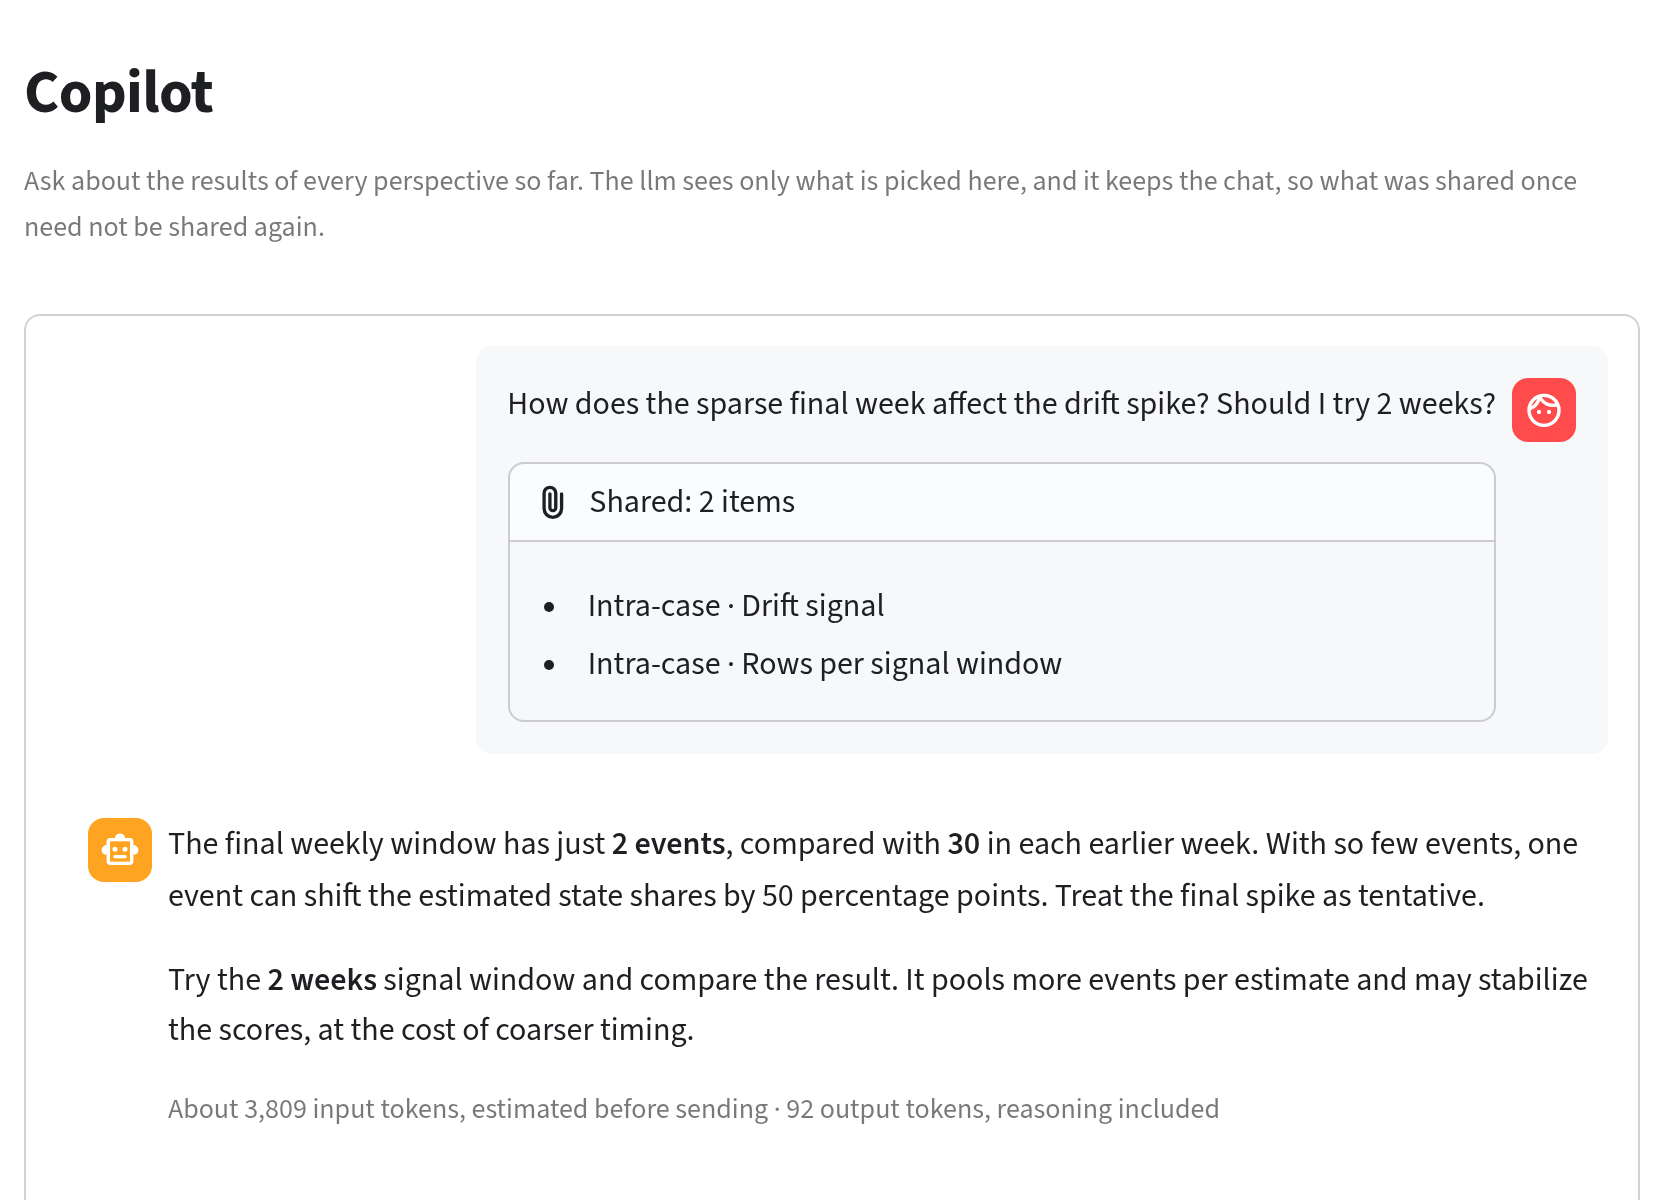
\includegraphics[width=0.8\textwidth]{figures/dashboard-copilot.png}
  \caption{Copilot review of a sparse signal window in a synthetic intra-case example. The analyst shares the drift summary and the observation-count plot. A local demonstration endpoint supplied the scripted reply.}
  \label{fig:implementation-copilot}
\end{figure*}

\paragraph{Configuration search with an analysis agent.}
A separate workflow, used in the thesis~\cite{kairo-thesis}, gives a tool-enabled agent an event log and an analysis objective. The agent uses event volume, time span, and available attributes to propose an initial configuration. It runs the library and uses the outputs to choose what to vary. For example, it can compare clustering settings on the same feature rows, inspect the observations behind peaks, and test whether a change remains visible with nearby window lengths or another reference. State profiles and feature shifts around candidate dates help explain which measurements account for a change. The workflow asks the agent to record the selected configuration, threshold, and drift signal for each analyzed perspective. It keeps annotated drift times out of the search.

Both workflows support parameter exploration. Their suggestions depend on the selected evidence and the model. In the thesis, agent-selected configurations yielded lower precision than configurations tuned by hand with access to drift annotations~\cite{kairo-thesis}. Analysts can review the suggested settings against the state distributions and the amount of data in the signal windows. The comparative benchmark in \autoref{sec:assessment} uses predefined configuration rules based on observed log properties and computes its scores and alarms without LLM assistance.
